\section{Measuring traffic streamed to server}

\subsection{Necessary Silent Gap}

As from the former result, we could see that Alexa would not be able to detect when the command ends and where to cut off once we started talking too quickly right after the command. Therefore, here raises another question is about how long should we pause before we start our conversation to let Alexa aware that the command is over and avoid Alexa transmitting our private conversation onto the Amazon server.

Here in the Fig. \ref{fig:gap}. The orange chunk means Alexa does not response anything to the sentence. The blue chunk means Alexa response to the whole sentence that made by us but did not know what does it mean. And the green chunk means Alexa had noticed the command and only replied to that part instead of the whole sentence. From Fig. \ref{fig:gap} we can draw out our main result is that we have to stop at least 0.7 seconds or more after the command ends to let the Alexa to figure out the command is over and not transmit any other voice data to the server.

\begin{figure}[ht]
	\centering
	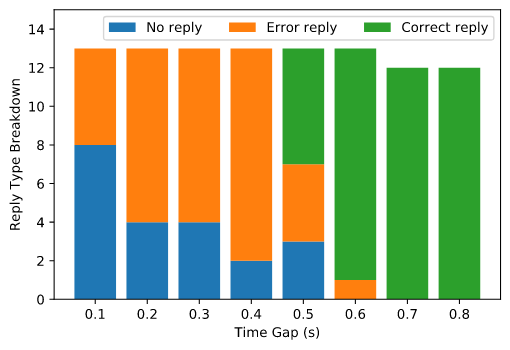
\includegraphics[scale=0.4]{../measurement/results/1207night/reply_type_breakdown}
	\caption{Bar plot showing how often Alexa replied correctly to a command for different gap lengths between the command and non-command speech.}
	\label{fig:gap}
	\vspace{-3mm}
	\end{figure}

To confirm our results, we extract the response package that Amazon server sent to Alexa and we could see a significant difference among "non-response" package, "error response" package and "correct response" package in Fig \ref{fig:postfix_variablegap_sizes}. The size of package ranged around a mean number for each specific response. The line means the size that the package ranges and the star in the middle of the line is the mean size of each type of packages. The orange one stands for "non-response" package, and the blue one stands for "error response" while the green one stands for "correct response" 

\begin{figure}[]
    \centering
    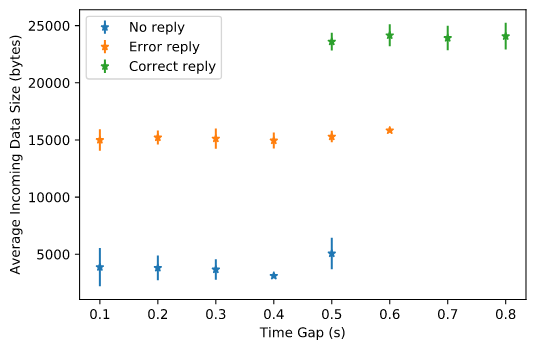
\includegraphics[width=\linewidth]{1207night/in_data_vs_gap_by_reply_type}
    \caption{Plot of the total outgoing data size against the length of the gap before non-command speech is played a command. The error bars extend to one standard deviation in either direction. Total outgoing data size is calculated as the sum of the TLS packet payload lengths going to the destination IP address with the greatest such sum.}
    \label{fig:postfix_variablegap_sizes}
\end{figure}

\subsection{How Alexa decided the end}

In the experiment \todo{[3]} we did an experiment to figure out how Alexa decided to stop transmitting and whether Alexa would raise privacy concern in three different kinds of situation in our life.

First, we played a background music while talking to Alexa and we found out that Alexa would stop transmitting package to Amazon server and start replying even though the music is still playing, which means Alexa can distinguish light music from human voice.

However, when we played the command voice with some conversation in the background and keep the conversation going after the command, we found out that Alexa would keep recording if there were no significant silent gap in the whole conversation, even though the conversation and command were generated by different people. As a result, Alexa is not able to detect different people's voice and stop automatically. This would suggest us not to say any private things when someone are using Alexa if we don't let them to be recorded. 

Further, when simulating the situation that few conversation happens around Alexa and someone waked up Alexa accidently, we played a full meaningless sentence with wake up word in the beginning and without any pause in it. The results turned out to be when we played a 18s sentence, the Alexa stops at 6s, 9s, 12s, 15s automatically before the sentence ends. We would assume that Alexa might stop at somewhere randomly. This result might prove that Alexa did try to protect our privacy once they figure out the voice is meaningless.

This measures the traffic streamed to server.


\begin{figure}[]
    \centering
    \includegraphics[width=\linewidth]{1204/outgoing_data_size_vs_prefix_time.png}
    \caption{Plot of the total outgoing data size against the length of non-command speech played immediately before a command. The error bars extend to one standard deviation in either direction. Total outgoing data size is calculated as the sum of the TLS packet payload lengths going to the destination IP address with the greatest such sum.}
    \label{fig:prefix_many}
\end{figure}

\begin{figure}[]
    \centering
    \includegraphics[width=\linewidth]{1205/outgoing_data_size_vs_prefix_time.png}
    \caption{\todo{Should probbaly be a bar graph, if present at all. Alternately, side-by-side histograms may be effective}. Plot of the total outgoing data size against the length of non-command speech played immediately before a command. The error bars extend to one standard deviation in either direction. Total outgoing data size is calculated as the sum of the TLS packet payload lengths going to the destination IP address with the greatest such sum.}
    \label{fig:prefix_two}
\end{figure}

\begin{figure}[]
    \centering
    \includegraphics[width=\linewidth]{1206/extra_filtered_outgoing_data_size_vs_prefix_time.png}
    \caption{\todo{Should probbaly be a bar graph, or maybe histograms, but I think three histograms is too many}. Plot of the total outgoing data size against the length of non-command speech played 0.5 s after a command. The error bars extend to one standard deviation in either direction. Total outgoing data size is calculated as the sum of the TLS packet payload lengths going to the destination IP address with the greatest such sum.}
    \label{fig:postfix_gap}
\end{figure}

\begin{figure}[]
    \centering
    \includegraphics[width=\linewidth]{1207/extra_filtered_outgoing_data_size_vs_prefix_time.png}
    \caption{Plot of the total outgoing data size against the length of non-command speech played immediately after a command. The error bars extend to one standard deviation in either direction. Total outgoing data size is calculated as the sum of the TLS packet payload lengths going to the destination IP address with the greatest such sum.}
    \label{fig:postfix_nogap}
\end{figure}


